\documentclass[border=10pt]{standalone}
\usepackage{tikz}
\usetikzlibrary{positioning, calc, matrix, fit, arrows.meta}
\begin{document}
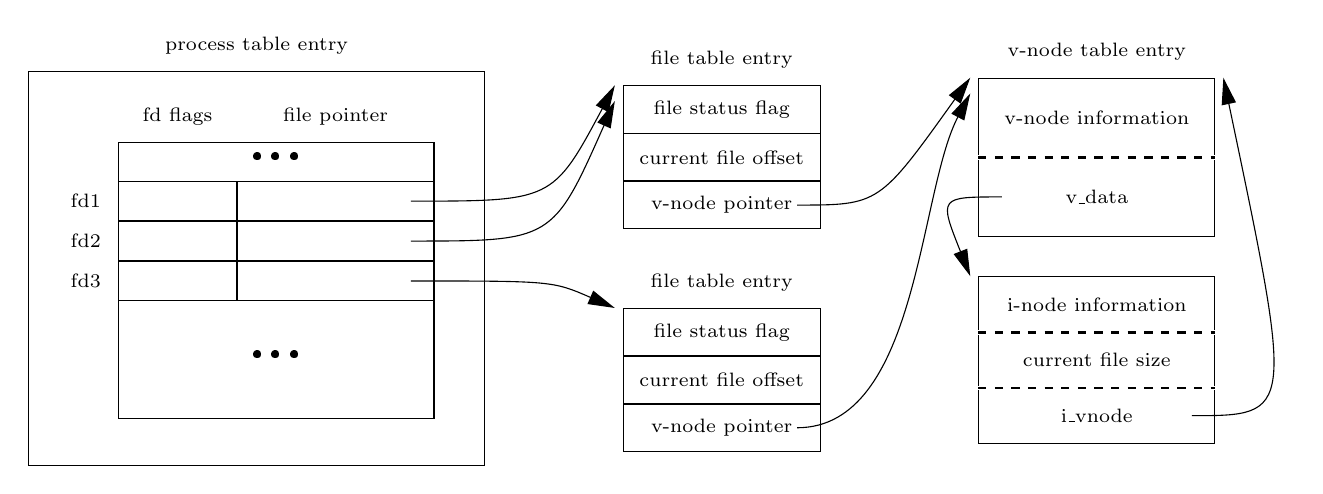
\begin{tikzpicture}[
  every node/.style={draw=none, font=\scriptsize}, % invisible border
  every matrix/.style={
    draw,
    matrix of nodes,
    nodes in empty cells,
    % inner sep=0, % Removes any inner padding within the matrix
    % the three sep setting make overlapping look neat
    row sep=+-.5\pgflinewidth,
    column sep=+-.5\pgflinewidth,
    inner sep=+-.5\pgflinewidth,
  },
  arrows={-{Stealth[inset=0pt, angle=30:10pt]}}, % tip angle:30°, dimension:10pt
  outer sep=auto,
]
  % process table entry
  \node[
    rectangle, draw, minimum width=58mm, minimum height=50mm
  ] (pte) at (0,0) {};
  %% label
  \node[above=1mm of pte] {process table entry};
  % file descriptor table
  \matrix[
    shift={(2.5mm,-1.5mm)}, % position, `anchor=center` is default
    nodes={draw, minimum height=5mm},
    column 1/.style={nodes={minimum width=15mm}},
    column 2/.style={nodes={minimum width=25mm}},
    row 1/.style={nodes={draw=none}},
    row 5/.style={nodes={draw=none, minimum height=15mm}},
  ](fdt) {
    % 1st row
       & \\
    % 2nd row
    {} & {} \\
    % 3rd row
    {} & {} \\
    % 4th row
    {} & {} \\
    % 5th row
       & \\
  };
  \node[fit=(fdt-1-1)(fdt-1-2)]{• • •}; % 1st row spans two cols
  \node[fit=(fdt-5-1)(fdt-5-2)]{• • •}; % 5th row spans two cols
  %% labels
  \node[above=1mm of fdt-1-1] {fd flags};
  \node[above=1mm of fdt-1-2] {file pointer};
  \node[left=1mm of fdt-2-1] {fd1};
  \node[left=1mm of fdt-3-1] {fd2};
  \node[left=1mm of fdt-4-1] {fd3};

  % file table entries
  \matrix[
    right=30mm of pte,
    anchor=south,
    shift={(0, 5mm)},
    nodes={draw, minimum height=6mm},
    column 1/.style={nodes={minimum width=25mm}},
  ](fte1) {
    {file status flag} \\
    {current file offset} \\
    {v-node pointer} \\
  };
  \node[above=1mm of fte1] {file table entry};

  \matrix[
    right=30mm of pte,
    anchor=north,
    shift={(0, -5mm)},
    nodes={draw, minimum height=6mm},
    column 1/.style={nodes={minimum width=25mm}},
  ](fte2) {
    {file status flag} \\
    {current file offset} \\
    {v-node pointer} \\
  };
  \node[above=1mm of fte2] {file table entry};

  % arrows from fp to fte
  \draw ($(fdt-2-2.east) - (3mm,0)$) .. controls 
    ($(fdt-2-2.east) + (15mm,0)$) .. ($(fte1.north west) - (1mm,0)$);
  \draw ($(fdt-3-2.east) - (3mm,0)$) .. controls
    ($(fdt-3-2.east) + (15mm,0)$) .. ($(fte1.north west) - (1mm,2mm)$);
  \draw ($(fdt-4-2.east) - (3mm,0)$) .. controls
    ($(fdt-4-2.east) + (15mm,0)$) .. ($(fte2.north west) - (1mm,0)$);

  % v-node table entry
  \matrix[
    right=20mm of fte1,
    nodes={draw, minimum height=10mm},
    column 1/.style={nodes={minimum width=30mm}},
  ](vnode) {
    {v-node information} \\
    {v\_data} \\
  };
  \node[above=1mm of vnode] {v-node table entry};

  %% dashed lines on white lines
  \draw[-,white,line width=2\pgflinewidth]
    (vnode-1-1.south west) -- (vnode-1-1.south east);
  \draw[-,dashed,line width=1.5\pgflinewidth]
    (vnode-1-1.south west) -- (vnode-1-1.south east);


  % i-node
  \matrix[
    below=5mm of vnode,
    nodes={draw, minimum height=7mm},
    column 1/.style={nodes={minimum width=30mm}},
  ](inode) {
    {i-node information} \\
    {current file size} \\
    {i\_vnode} \\
  };

  %% dashed lines on white lines
  \draw[-,white,line width=2\pgflinewidth]
    (inode-1-1.south west) -- (inode-1-1.south east);
  \draw[-,dashed,line width=1.5\pgflinewidth]
    (inode-1-1.south west) -- (inode-1-1.south east);
  \draw[-,white,line width=2\pgflinewidth]
    (inode-2-1.south west) -- (inode-2-1.south east);
  \draw[-,dashed,line width=1.5\pgflinewidth]
    (inode-2-1.south west) -- (inode-2-1.south east);

  % arrows from fte to v-node
  \draw ($(fte1-3-1.east) + (-3mm,0)$) .. controls
    ($(fte1-3-1) + (20mm,0)$) .. ($(vnode.north west) - (1mm,0)$);
  \draw ($(fte2-3-1.east) + (-3mm,0)$) .. controls
    ($(fte2-3-1) + (25mm,0)$) and ($(fte2-3-1) + (25mm,30mm)$)
    .. ($(vnode.north west) - (1mm,2mm)$);

  % arrows from v-node to i-node
  \draw ($(vnode-2-1.west) + (3mm,0)$) .. controls
    ($(vnode-2-1.west) - (5mm,0)$) .. ($(inode.north west) - (1mm,0)$);
  % arrows from i-node to v-node
  \draw ($(inode-3-1.east) + (-3mm,0)$) .. controls
    ($(inode-3-1.east) + (10mm,0)$) .. ($(vnode.north east) + (1mm,0)$);

\end{tikzpicture}
\end{document}
